\documentclass[a4paper]{article} 
\addtolength{\hoffset}{-2.25cm}
\addtolength{\textwidth}{4.5cm}
\addtolength{\voffset}{-3.25cm}
\addtolength{\textheight}{5cm}
\setlength{\parskip}{0pt}
\setlength{\parindent}{0in}

%----------------------------------------------------------------------------------------
%	PACKAGES AND OTHER DOCUMENT CONFIGURATIONS
%----------------------------------------------------------------------------------------

\usepackage{blindtext} % Package to generate dummy text
\usepackage{charter} % Use the Charter font
\usepackage[utf8]{inputenc} % Use UTF-8 encoding
\usepackage{microtype} % Slightly tweak font spacing for aesthetics
\usepackage[english, ngerman]{babel} % Language hyphenation and typographical rules
\usepackage{amsthm, amsmath, amssymb} % Mathematical typesetting
\usepackage{float} % Improved interface for floating objects
\usepackage[final, colorlinks = true, 
            linkcolor = black, 
            citecolor = black]{hyperref} % For hyperlinks in the PDF
\usepackage{graphicx, multicol} % Enhanced support for graphics
\usepackage{xcolor} % Driver-independent color extensions
\usepackage{marvosym, wasysym} % More symbols
\usepackage{rotating} % Rotation tools
\usepackage{censor} % Facilities for controlling restricted text
\usepackage{listings, style/lstlisting} % Environment for non-formatted code, !uses style file!
\usepackage{pseudocode} % Environment for specifying algorithms in a natural way
\usepackage{style/avm} % Environment for f-structures, !uses style file!
\usepackage{booktabs} % Enhances quality of tables
\usepackage{tikz-qtree} % Easy tree drawing tool
\tikzset{every tree node/.style={align=center,anchor=north},
         level distance=2cm} % Configuration for q-trees
\usepackage{style/btree} % Configuration for b-trees and b+-trees, !uses style file!
\usepackage[backend=biber,style=numeric,
            sorting=nyt]{biblatex} % Complete reimplementation of bibliographic facilities
\addbibresource{ecl.bib}
\usepackage{csquotes} % Context sensitive quotation facilities
\usepackage[yyyymmdd]{datetime} % Uses YEAR-MONTH-DAY format for dates
\renewcommand{\dateseparator}{-} % Sets dateseparator to '-'
\usepackage{fancyhdr} % Headers and footers
\pagestyle{fancy} % All pages have headers and footers
\fancyhead{}\renewcommand{\headrulewidth}{0pt} % Blank out the default header
\fancyfoot[L]{} % Custom footer text
\fancyfoot[C]{} % Custom footer text
\fancyfoot[R]{\thepage} % Custom footer text
\newcommand{\note}[1]{\marginpar{\scriptsize \textcolor{red}{#1}}} % Enables comments in red on margin

%----------------------------------------------------------------------------------------

\begin{document}


%-------------------------------
%	TITLE SECTION
%-------------------------------

\fancyhead[C]{}
\hrule \medskip % Upper rule
\begin{minipage}{0.295\textwidth} 
\raggedright
\footnotesize
Sofia Caltabiano \hfill\\  
Martina Chiesa \hfill\\ 
Simon Cotterill \hfill\\
Muyang Li \hfill\\
Lisa Skelton \hfill\\
Josiah Tsang \hfill\\
\end{minipage}
\begin{minipage}{0.4\textwidth} 
\centering 
\large 
Project proposal EEG\\ 
\normalsize 
Manufacturing Engineering, 465\\ 
\end{minipage}
\begin{minipage}{0.295\textwidth} 
\raggedleft
\today\hfill\\
\end{minipage}
\medskip\hrule 
\bigskip

%-------------------------------
%	CONTENTS
%-------------------------------

\section{Motivation}

One of the most impressive aspects of Machine Learning and Artificial Intelligence (AI) is the ability to understand the relationship between handedness and BCI (Brian Computer Interface). Our goal is to understand how brainwave data within humans influences our decision to establish hand dominance using Machine Learning and AI.\\

The hand dominance effect is an essential characteristic of hemispheric specialization in the human motor system. Independent of cultural and historical backgrounds, around 90\% of humans prefer to use their right hand for skilled manipulation. ({\href{https://www.nature.com/articles/s41598-021-87396-4}{Hand preference for the visual and auditory modalities in humans}}) Understanding the brainwave of hand dominance is important for building a Brain-computer interface (BCI) as studies have suggested that handedness could contribute to the performance variations of BCI, especially when implementing motor imagery (MI) tasks.  ({\href{https://pubmed.ncbi.nlm.nih.gov/31918621/}{Brain–computer interface performance analysis of monozygotic twins with discordant hand dominance: A case study}}) Specifically, studies show the power of sensorimotor rhythms (SMR) measured differs according to handedness. The Sensorimotor Rhythm (SMR) is an oscillatory idle rhythm of synchronized electric brain activity with a brainwave frequency between alpha and beta waves (12-15 Hz).  ({\href{https://pubmed.ncbi.nlm.nih.gov/7691544/}{Functional significance of the mu rhythm of human cortex: an electrophysiologic study with subdural electrodes}})\\

Application of data obtained in our study could help inform a variety of areas by correlating EEG signals to hand dominance. Only 10\% of the population is left hand dominant, and through this study we will learn more about the ways in which left hand dominant persons brain activity differs from right hand dominant individuals. It is established that handedness is correlated with hemispheric language centers. A mix of scientific and anecdotal evidence exists correlating other attributes to hemispheric regions including spatial awareness, creativity, language and logic.This study may assist in providing quantifiable metrics to the differences in brain activity based on hand dominance with potential application in neurology, brain injury recovery, stroke recovery and more.\\

Furthermore, any problem that affects the brain manifests differently depending on whether a person is right-handed or left-handed. So, knowing which is the dominant part of the brain is useful in many medical areas. For example, in neurological science, when a person needs to undergo a brain operation, it is important for the surgeon to know which is the dominant part of the brain. This helps them avoid causing permanent damage in integral areas.\\

%\bigskip

%------------------------------------------------

\section{Objective} 

The objective of this study is to use machine learning models to predict the dominant hand of a person using brainwave data collected by the MUSE 2.  Muse 2 is a multi-sensor electroencephalograph (EEG) device that provides real-time biofeedback on brain activity, heartbeat, breathing, and movement by attaching a set of electrodes to the scalp to measure the electrical activity of the brain.\\

For every EEG recorded, we will obtain a very high number of features, which will be reduced and analyzed during the preprocessing step. Then some Machine Learning algorithms for classification will be used to predict the class of a future unseen EEG wave.\\

This study will be conducted not only to understand the differences in the behavior of our brain when using the dominant or the weak arm, but also to see the analogies and differences in the effort required when doing a simple action (which should require less concentration) compared to a complicated action.\\

%\bigskip

%------------------------------------------------

\section{Collecting data}

For data collection, the testing per person should take less than 10 minutes. Keeping this time short will allow for fast data collection and make it easier to find willing participants.\\

As advised by our TA, our experiment would ideally have 4 classes: casual writing and intensive writing for both the dominant and nondominant hands. Assuming each test takes 2 minutes, we could have 2 tests for casual writing, 2 tests for intensive writing, and 2 minute left over for cleaning the MUSE and instructing participants.\\

For our casual writing tests, we will ask participants to checkmark a series of boxes and scribble in a large circle. For our first intensive writing tests, we will ask participants to rewrite a sentence and copy a series of unfamiliar figures, like written Mandarin for a non-native speaker.\\

Assuming we can keep testing to 10 minutes per individual, we would be able to conduct 6 tests per hour. We hope to conduct a minimum of 45 tests, or roughly 9 testing periods of 1 hour.\\

%\bigskip

%------------------------------------------------

\section{Data analysis}

We will build several machine learning models with the purpose to classify new observations. Classification models we have considered to be successful for training the model include Linear Discriminant Analysis (LDA), Support Vector Machine (SVM), and deep learning Neural Network (NN) based on absolute and relative brainwaves. Moreover, we also believe that utilizing unsupervised learning algorithms such as K-Nearest Neighbor (KNN) or Artificial Neural Network (ANN) to create groups will achieve improved performance.\\

%\bigskip

%------------------------------------------------

\section{Plan}

A gantt chart has been created to govern the overall timeline and task distribution of this project.
({\href{https://docs.google.com/spreadsheets/d/1qmQjmoMOXTPG9QAKZYcwapSyiNY8_c84OKD3P4-Kbx8/edit#gid=0}{Gantt chart}})\\
\begin{figure}[H]
    \centering
    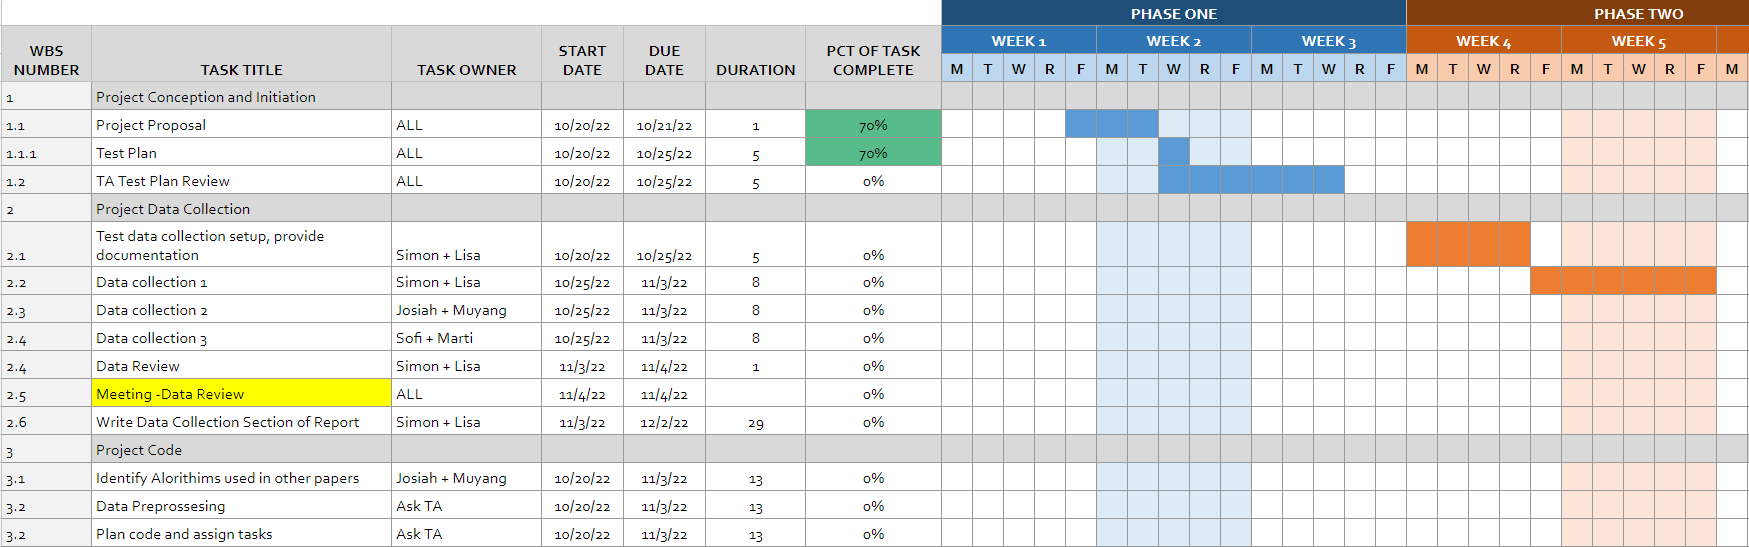
\includegraphics[width=10cm]{Gantt}
    \label{fig:galaxy}
\end{figure}

The team will test over 3 days, and split into 3 pairs with each pair setting up according to the data Collection protocol devised by Simon \& Lisa. Testing will take place between October 25 and November 3rd. Each pair will test a minimum of 15 participants for a total of 45 (minimum).\\

The setup will be in a distraction free environment and will require:
\begin{center}
\begin{tabular}{ c c c c}
 Desk & 3 Chairs & Laptop & Muse device \& App \\ 
 Writing utensil & Test Template & Alcohol sanitizing wipes & Hand sanitizer   
\end{tabular}
\end{center}

%\subsection{Safety and Security}
\textbf{Safety and Security}
We will ask participants pre-screening questions prior to engaging in testing to limit the spread of Covid-19. Potential participants who experience symptoms or may have recent exposure will be declined.\\

Participants will be asked to sanitize their hands prior to starting the test and the Muse device will be thoroughly cleaned with alcohol wipes between uses.\\

%\subsection{Project Management}
\textbf{Project Management}
We will be using GitHub for version control and storage of all project related code.  This repository can be shared with the professor and TA’s if requested.\\

%------------------------------------------------

\end{document}
